\documentclass[7pt,twocolumn]{article}

\usepackage[a4paper, margin={.3in, .3in}]{geometry}
\usepackage{latexsym,graphicx}
\usepackage{amsmath,amssymb}
\usepackage{amsthm}
\usepackage{enumerate}
\usepackage{graphicx}
\usepackage{cleveref}
\usepackage{algorithmic}
\usepackage{algorithm}
\usepackage{color}

% Useful macros
\newcommand{\E}[1]{\mathbf{E}\l[#1\r]}
\newcommand{\problem}[1]{\section*{Problem #1}}
\renewcommand{\l}{\left}
\renewcommand{\r}{\right}
\renewcommand{\iff}{\Leftrightarrow~}
\newcommand{\intff}{\int_{-\infty}^\infty }
\newcommand{\intzf}{\int_0^\infty }
\newcommand{\intpp}{\int_{-\pi}^\pi }
\newcommand{\sumzf}[1]{\sum_{#1=0}^\infty}
\newcommand{\sumff}[1]{\sum_{#1=-\infty}^\infty}
\newcommand{\Bin}{\text{Bin}}
\newcommand{\pfrac}[2]{\l(\frac{#1}{#2}\r)}
\renewcommand{\bf}{\textbf}
\newcommand{\zm}[1]{z^{-#1}}
\renewcommand{\P}[1]{\mathbf{P}\l\{#1\r\}}
\newcommand{\Var}[1]{\mathbf{Var}\l(#1\r)}
\newcommand{\Poiss}{\text{Poiss}}
\newcommand{\Geom}{\text{Geom}}
\newcommand{\Skew}{\text{\bf{Skew}}}

\newtheorem{lemma}{Lemma}
\newtheorem{theorem}[lemma]{Theorem}
\newtheorem{informaltheorem}[lemma]{Informal Theorem}
\newtheorem{informallemma}[lemma]{Informal Lemma}
\newtheorem{corollary}[lemma]{Corollary}
\newtheorem{definition}[lemma]{Definition}
\newtheorem{proposition}[lemma]{Proposition}
\newtheorem{question}{Question}
\newtheorem{example}[lemma]{Example}
\newtheorem{remark}[lemma]{Remark}
\newtheorem{claim}{Claim}
\newtheorem{fact}{Fact}
\newtheorem{challenge}{Challenge}
\newtheorem{observation}{Observation}
\newtheorem{openproblem}{Open Problem}
\newtheorem{openquestion}{Open question}

\newcommand{\beq}{\begin{equation}}
\newcommand{\eeq}{\end{equation}}
\newcommand{\beas}{\begin{eqnarray*}}
\newcommand{\eeas}{\end{eqnarray*}}

\newcommand{\poly}{\mathrm{poly}}
\newcommand{\eps}{\epsilon}
\newcommand{\e}{\epsilon}
\newcommand{\polylog}{\mathrm{polylog}}
\newcommand{\rob}[1]{\left( #1 \right)} %Round Brackets
\newcommand{\sqb}[1]{\left[ #1 \right]} %square Brackets
\newcommand{\cub}[1]{\left\{ #1 \right\} } %curly brackets
\newcommand{\rb}[1]{\left( #1 \right)} %Round
\newcommand{\abs}[1]{\left| #1 \right|} %| |
\newcommand{\zo}{\{0, 1\}}
\newcommand{\zonzo}{\zo^n \to \zo}
\newcommand{\zokzo}{\zo^k \to \zo}
\newcommand{\zot}{\{0,1,2\}}
\newcommand{\norm}[1]{\left\lVert#1\right\rVert}
%
%\newcommand{\en}[1]{\marginpar{\textbf{#1}}}
%\newcommand{\efn}[1]{\footnote{\textbf{#1}}}
\newcommand{\bR}{\mathbb{R}}
\newcommand{\bE}{\mathbb{E}}
\newcommand{\bN}{\mathbb{N}}

\newcommand{\define}[2]{{\large \textbf{#1}} #2}
\pagenumbering{gobble}
\setlength\parindent{0pt}
\newcommand{\todo}[1]{\textbf{\color{red} TODO: #1}}

\usepackage{titlesec}
\titlespacing*{\section}{0pt}{2pt}{2pt}

%%%%%%%%%%%%%%%%%%%%%%%%%%%%%%%%%%%%%%%%%%%%%%%%%%%%%%%%%%%%%%%%

\begin{document}
\setlength{\abovedisplayskip}{.3em}
\setlength{\belowdisplayskip}{.3em}

\section{Definitions}

\define{CSMA/CD}{Carrier Sense Multiple Access with Collision Detection}
\define{CSMA/CA}{Carrier Sense Multiple Access with Collision Avoidance}
\define{SDMA}{Space Division Multiple Access}
\define{TDMA}{Time Division Multiple Access}
\define{FDMA}{Frequency Division Multiple Access}
\define{CDMA}{Code Division Multiple Access}
\define{DAMA}{Demand Assigned Multiple Access}
\define{MACA}{Multiple Access with Collision Avoidance}
\define{RTS}{request to send}
\define{CTS}{clear to send}
\define{BSS}{Basic Service Set}
\define{DCF}{distributed coordination function}
\define{SNR}{Signal to noise ratio}
\define{ISI}{Inter symbol interference}
\define{COA}{Care of Address}
\define{HA}{Home Agent}
\define{FA}{Foreign Agent}
\define{MPTCP}{Multi Path TCP}
\define{ERP}{Effective Radiated Power}
\define{LOS}{Line of sight}
\define{DIFS}{Distributed Inter-Frame Space time (SIFS + 2 slot time)}
\define{SIFS}{Short Inter-Frame Space time}
\define{CW}{Contention window}
\define{NAV}{Net Allocation Vector}
\define{EIFS}{Extended Inter-Frame Space time (SIFS + ACK$_{t}$ + DIFS time)}
\define{ST}{Slot Time}
\define{CS}{Collision Sensing}
\define{CD}{Collision Detection}
\define{HIP}{Host Identity Protocol}
\define{ICMP}{Internet Control Message Protocol}
\define{GAN}{Generic Access Network}
\define{IMSI}{International Mobile Subscriber Identity}
\define{TMSI}{Temporary Mobile Subscriber Identity}
\define{SACK}{Selective ACK}

% PIFS = SISF + 1 slot time

\section{WLAN}

\bf{Delays rule of thumb.} Wait DIFS without activity before RTS, then wait SIFS between packages

\bf{802.11 MAC layer CSMA/CA.} The following mechanism is called \emph{exponential back off}. If the channel is busy for the source, a back off time (measured in slot times) is chosen randomly in the interval $[0,CW)$. This timer is decreased by one as long as the channel is sensed idle for a DIFS. The timer stops when the channel is busy and resumes when the channel is idle again for at least a DIFS period. $CW$ is an integer whose range is determined by the PHY layer characteristics: $CW_{min}$ and $CW_{max}$. $CW$ is doubled after each unsuccessful transmission, up to the maximum value equal to $CW_{max} + 1$. When the back off timer reaches zero, the source transmits the data packet. The ACK is transmitted by the receiver immediately after a period of duration equal to SIFS. When a data packet is transmitted, all other stations hearing this transmission adjust their NAV. The NAV maintains a prediction of future traffic on the medium based on the duration information that is announced in Data frames (or RTS/CTS). In addition, whenever a node detects an erroneous frame, the node defers its transmission by a fixed duration indicated by EIFS. $CW$ is doubled for each collision (failed transmission). In case of a successful (i.e. collision-free) transmission, the transmitting station brings the value of its contention window back to $CW_{min}$. 


Given A - B - C configuration

\bf{Hidden terminal.} A transmit to B, C sense free medium (CS fails) and transmit to B, collision at B and A does not see it (CD fails).

\bf{Exposed terminal.} B sends to A, C wants to send to another terminal, C has to wait (because CS) while it could transmit because not in A radio range.

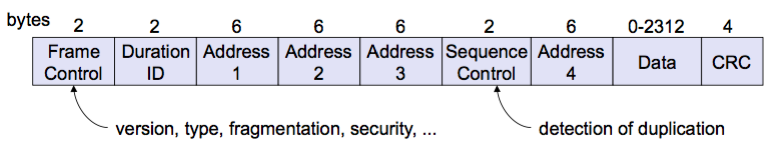
\includegraphics[width=\linewidth]{figures/package-frame-1.png}

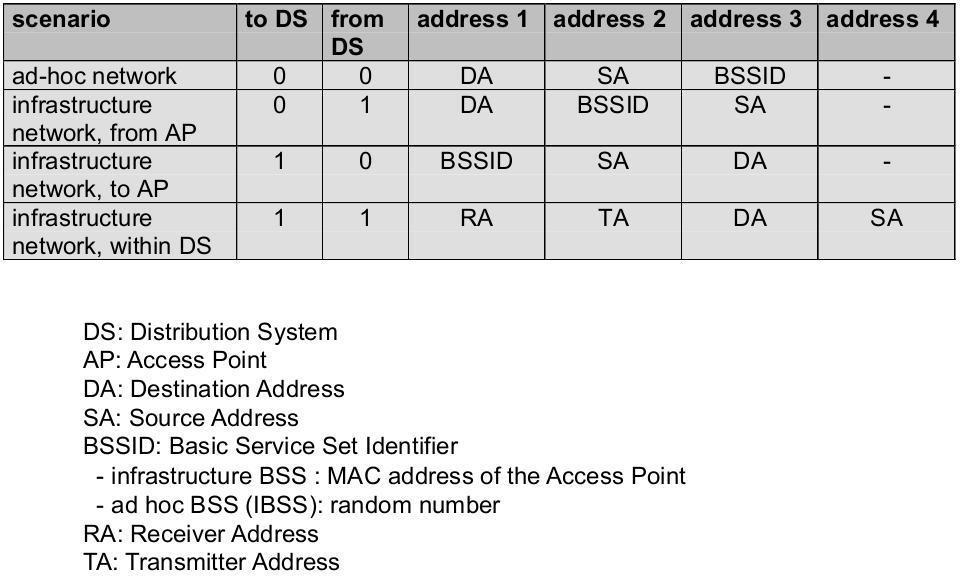
\includegraphics[width=\linewidth]{figures/package-frame-2.png}

\section{TCP performance}

\bf{Aloha Protocol.} Send package and wait for ACK, if timeout $2 t_{prop}$ then back off time $B$ and retry. 


Given that $S$ is the output rate and $G$ is the input rate

\bf{Aloha performance.} $S = Ge^{-2G}$ peakvalue at $G=1/2$, $S=1/2e$, $\E{T} / X = 1 + a + (e^{2G} - 1)(1 + 2a + B/X)$ with $a=t_{prop}/X$

\bf{Slotted aloha performance.} $S = Ge^{-G}$ peakvalue at $G=1$, $S=e^{-1}$, $\E{T} / X = 1 + a + (e^G - 1)(1 + 2a + B/X)$

\bf{CSMA persistent.} \emph{1-persistent} send when idle, back off if collision, \emph{non-persistent} transmit if idle else back off, \emph{$p$-persistent} if busy re sense else if idle transmit with proba $p$, re sense after random delay with proba $1-p$

\begin{figure}
  \centering
  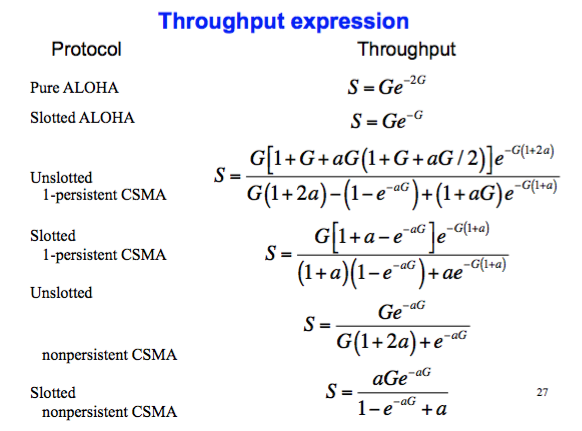
\includegraphics[width=0.8\linewidth]{figures/throughput.png}
\end{figure}

\bf{MPTCP.} use Dseq and Dack for real sequence number instead of seq tag to avoid middle box drop some packages

\bf{MPTCP Congestion control.} When receive ACK for flow $r$, increase $w_r$ by 
\[
  \min_{S\subseteq R: r\in S} \frac{\max_{s\in S}w_s / RTT_s^2}{\l( \sum_{s\in w_s}/ RTT_s \r)^2}
\]
otherwise divide window size by 2

\section{Bianchi Model}

% 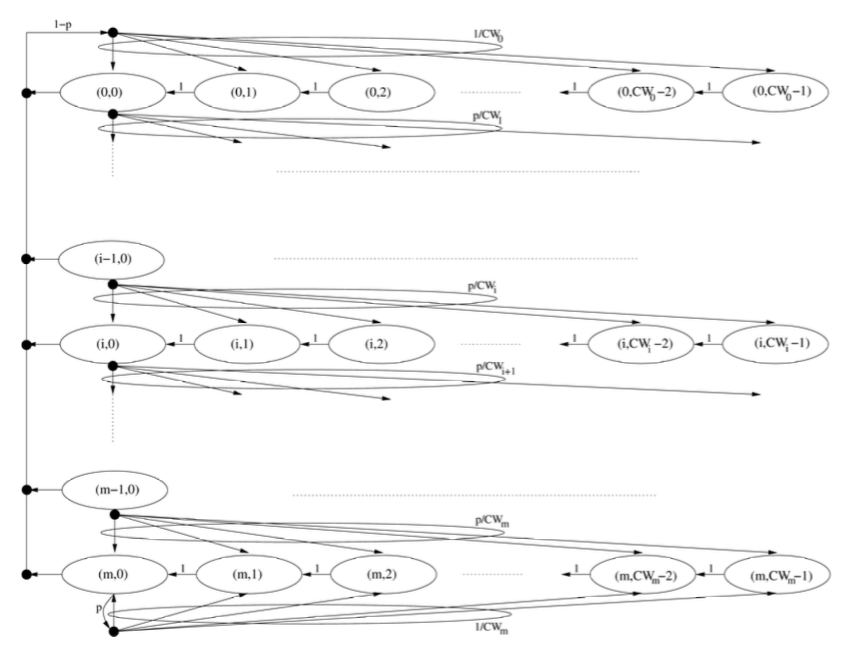
\includegraphics[width=\linewidth]{figures/bianchi-model.png}

Bianchi uses a two-dimensional Markov chain of m + 1 back off stages in which each stage represents the back off time counter of a node. 

$p$ is the probability that, in a slot time, at least one of the $N-1$ remaining stations transmits as well $p=1-(1-\pi)^{N-1}$

Probability that a station transmits in a randomly chosen slot time $\pi = \sum_{i=0}^m b_{i,0}$

Markov chain stationary distribution:
\[
  b_{i,k} = \frac{CW_i - k}{CW_i} \cdot \begin{cases}
    (1-p) \sum_{j=0}^m b_{j,0} & i = 0\\
    p \cdot b_{i-1,0} & 0 < i < m \\
    p\cdot(b_{m-1,0}+b_{m,0}) & i = m
  \end{cases}
\]
\[
  \pi = \frac 2 {1+W_{min} + p W_{min} \sum_{k=0}^{m-1}(2p)^k}
\]


\bf{Saturation throughput.} 
$
  \tau = \frac{\E{\text{info transmitted in ST}}}{\E{\text{duration ST}}}$

\[= \frac {P_s P_{tr} L} {P_s P_{tr}T_s + P_{tr}(1-P_s)T_c + (1-P_{tr})T_{id}}\]

with $P_{tr} = 1 - (1-\pi)^N$ the proba there is $\geq 1$ transmission in a ST, $L$ average packet size, $T_s$ average time to transmit package size $L$ including SIFS, $P_s = \frac{N\pi(1-\pi)^{N-1}}{1-(1-\pi)^N}$ the proba of successful transmission, $T_{id}$ is the duration of the idle period (a single slot time); and $T_c$ is the average time spent in the collision.

\bf{Basic transmission mode.}
\[
  \begin{cases}
    T_s = H+L+SIFS+\sigma+ACK+DIFS+\sigma\\
    T_c = H + L + DIFS + \sigma
  \end{cases}
\]

\bf{RTS/CTS transmission mode.}
\[
  \begin{cases}
    T_s = RTS+3SIFS+4\sigma+CTS+H+L+ACK+DIFS\\
    T_c = RTS + DIFS + \sigma
  \end{cases}
\]

\section{Antennas}

\bf{to dB} $10 \log x$ \bf{from dB} $10^{y/10}$

\textbf{Power low for propagation} $P_r = c P_t d^{-\alpha}$ with $d$ in m and $\alpha$ often 2 or 4

\textbf{Free space omni directional} $P_R = P_T \frac{A_R}{4\pi d^2}\eta_R$

\textbf{Free space directional} $P_R = G_T P_T \frac{A_R}{4\pi d^2}\eta_R$

\textbf{Antenna gain} $G_T =\eta_T \frac{4\pi A_T}{\lambda^2}$

\textbf{Parabolic antenna gain} $G=7A/\lambda^2$

\textbf{Free space all directional received power} \\$P_R = P_T G_T G_R \pfrac{\lambda}{4\pi d}^2$


\textbf{ERP} $P_T \cdot G_T W$

\bf{Thermal Noise} in a bandwidth of 1Hz $N_0 = kT (W)$ 

\bf{Thermal Noise} in a bandwidth of BHz $N_0 = BkT (W)$ 

\bf{Boltzmann constant} $ k = 1.3803 \cdot 10^{-23} J\cdot K^{-1}$

\bf{Bit power to noise ratio}
\[
  \frac{E_b}{N_0}=\frac{P_R}{kTR}
\]

where $R$ is the communication bit rate, and $T$ the temperature of the receiver

\bf{Optical line of sight} $d = 3.57\sqrt h$

\bf{Radio LOS} $d = 3.57\sqrt {Kh}$, $K \approx 4/3$, $d$ in km

\bf{2 antennas LOS} $3.57(\sqrt{Kh_1} + \sqrt{Kh_2})$

\section{Cellular Networks}


\textbf{Surface hexagon} $A = \frac{3\sqrt 3} 2 R^2$

\bf{Radio capacity} $m = C/N$

\bf{Hexagon model} $Q=D/R = \sqrt{3N}$ where $D$ is the distance between two cells of same channel, $R$ the radius of a cell

\bf{Hexagon cell count} $N=i^2+ij+j^2, (i,j) \in \bN^2$ that is $1,3,4,7,9,12,13,16...$

\section{Privacy}

Poisson distribution assumption
$
  \P{k \text{ in } t \text{ range}} = \frac{t^k}{k!}e^{-t}
$


Hungarian algorithm (complexity: $O(n^4)$) on a weighted bipartite graph

\textbf{Tracking game}: Adversary picks vehicle $v$ in observed zone, tracks until enters mix zone at port $s$. With port $j$ and exiting time $t$, decide for $v'$ with max $q_{jt} = p_{sj}d_{sj}(t)$, with $p_{sj} = P\{\text{exiting at } j | \text{entering at } s\}$ and $d_{sj}(t)$ the prob that the time elapsed between entering $s$ and exiting $j$ is $t$.

\section{Security}

\bf{IPsec.} Provides confidentiality, authentication and integrity

\bf{GSM.} confidentiality of communications, encryption key established with help of home network (HN), short-term temporary identifiers for protection of the subscriber’s identity. Triplet ($K_c$, Rand, S) created by HN from IMSI, VN ask to authenticate Rand (with $K_i$) then use $K_c$. Problems: does not address active attacks, whereby some network elements (e.g. BTS: Base Station)

\bf{SIM card.} Contains IMSI, PIN, TMSI, $K_i$ user's secret key, $K_c$ cyphering key

\bf{WEP.} STA needs to authenticate itself to the AP based on a simple challenge-response protocol, use RC4 protocol, need IV. Two kinds of keys: default key, key mapping keys (better). Then association. \emph{Default keys}: same for group, when member leaves, change key.  Impossible to do simultaneously, so support multiple keys (one active + others). Flaws: authentication is one-way only, AP is not authenticated to STA, the same shared secret key is used for authentication and encryption, no session key is established during authentication (replay possible). For integrity ICV (integrity check value) appended then encrypted with message.

\section{Mobile TCP}

\bf{HIP.} New layer between IP and transport layer, architecture change

\bf{Mobile IP.} Adaptation of TCP for mobility. Three phases
\begin{enumerate}
  \item \bf{Agent discovery:} HA, FA periodically send ad messages, MN listens, if FA get a COA. It can request with broadcast solicitation message.
  \item \bf{Registration:} MN (COA) $\to$ FA $\to$ HA $\to$ FA $\to$ MN
  \item \bf{Tunneling:} IP in IP encapsulation
\end{enumerate}

\bf{Optimization.}  HA provides the CN with the current location of MN (FA) - Optimization of FA handover,  new FA informs old FA to avoid packet loss, old FA now forwards remaining packets to new FA - reverse tunneling

\bf{IPv6.} Security mandatory, "soft" hand-over, No FA COA is always co-located.

\bf{TCP Reno.} Window size set to 1 when timeout, divided by 2 when triple duplicated ACK. Slow start threshold = when to stop exponential increasing (for linear). If packet loss then slow start threshold = window size / 2. 

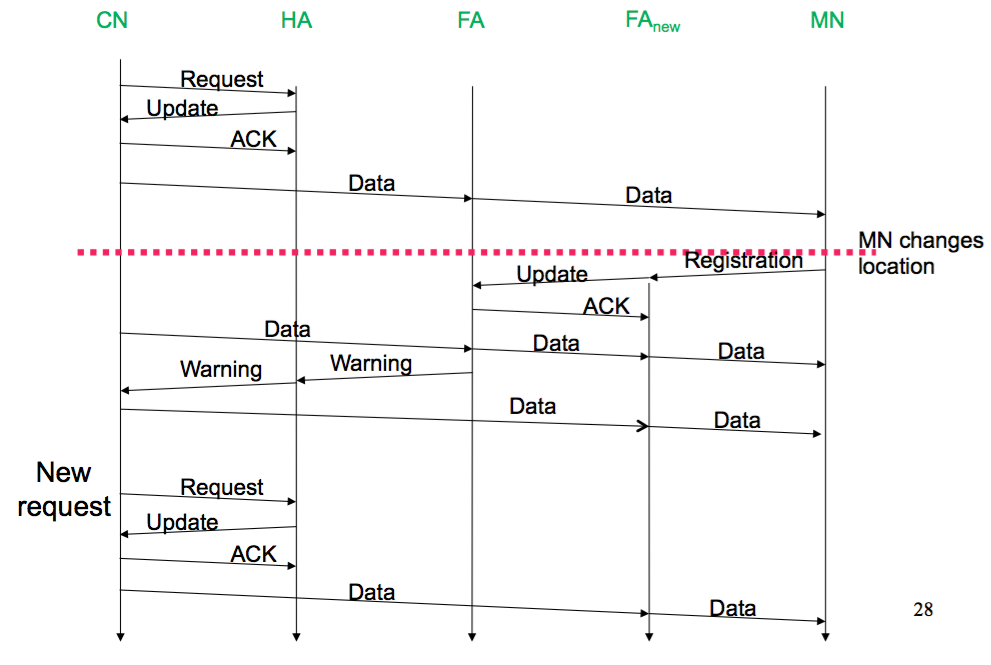
\includegraphics[width=\linewidth]{figures/mobile-ip-handover.png}

\end{document}
